% 06_confinement.tex -- Part 6, quantum confinement of crystalline In2O3 films. Sources: research_monograph/chapters/
% M05_confinement_theory.tex (envelope, Kane, finite barrier V4, partition V3, HSE ratio, subband spacing),
% M09_masses_parameters.tex (tab:mono-mass-laws, HSE-corrected gaps), 13_dft_rev.tex (stages 4b, 4c, 5;
% tab:dft-hse, tab:dft-partition, sec:mono-dft-thin), evidence/FACT_REGISTRY.tsv (FACT-002, 010*, 011*, 012-025,
% 028-032), evidence/derived/confinement_analysis.json, appendices/MG_corrections.tex (V3, V4).
% Figures: tools/fig_06_confinement.py (data: qe_workflow/analysis_2026-10-13_full/bands_masses/out/b03_gaps_laws.json,
% evidence/derived/confinement_analysis.json, tables/THICKNESS_LAW_EVIDENCE.csv for the gaps of Lin et al.).
% Note: frame bodies start with a command, never with a brace group (beamer would read a subtitle).
% Naming: "C10" is the frozen device-model law of campaign C10 (the monograph's "V3/C10" law); "V1" is the first device
% model (Part 4). The correction IDs V3/V4 of MG_corrections are not used on the slides.
\partslide{Part 6}{Quantum confinement of crystalline \InO{} films}

% denser slides: footnotesize bullets, local to the frame in which it is called
\providecommand{\sixdense}{\setbeamerfont{itemize/enumerate body}{size=\footnotesize}%
  \setbeamerfont{itemize/enumerate subbody}{size=\footnotesize}}
% evidence label inside a \src line: same wording as \lab, but keeps the small size of the source line
\providecommand{\sixlab}[1]{{\color{inkgrey}[\textsc{\MakeLowercase{#1}}]}}

% ---------------------------------------------------------------------------------------------------------------------
\begin{frame}{Four relaxed films; the two thinnest are special cases}
  \sixdense
  \begin{columns}[T,onlytextwidth]
    \begin{column}{0.59\textwidth}
      \begingroup\scriptsize
      \renewcommand{\arraystretch}{1.05}
      \setlength{\tabcolsep}{4pt}
      \begin{tabular}{@{}l l l c c >{\raggedright\arraybackslash}p{19mm}@{}}
        \toprule
        name & $\tHH$ (nm) & cell & $\Eg$ (eV) & $\dEg$ (eV) & role \\
        \midrule
        0.51\,nm & 0.461 & In$_8$(OH)$_{24}$ & 3.140 & $+2.251$ & excluded \\
        0.75\,nm & 0.695 & In$_{16}$O$_{36}$H$_{24}$ & 2.199 & $+1.310$ & polar; $\dEg$, $\Delta m$, frozen C10 $\dEc$ \\
        1\,nm & 0.930 & In$_{24}$O$_{48}$H$_{24}$ & 1.789 & $+0.900$ & all laws \\
        2\,nm & 1.962 & In$_{56}$O$_{96}$H$_{24}$ & 1.224 & $+0.335$ & all laws \\
        \bottomrule
      \end{tabular}\par\endgroup
      \src{Name: nominal thickness, used in the text; $\tHH$: relaxed H--H thickness. Recipe of Lin
        et al.\sref[p.~21542]{Lin2022}, relaxed; PAW-PBE; bulk gap 0.8887\,eV. This work \sixlab{computed}.}
      \begin{itemize}
        \item 0.461\,nm, one cation plane: all O bonded to H \lab{computed}.
        \item 0.695\,nm, two cation planes: inequivalent faces, no dipole correction\sref{Bengtsson1999}; the
          $-13.6$\,meV/\AA{} vacuum ramp gives $\dEc$ a $\pm0.17$\,eV reference sensitivity \lab{assumed}.
        \item Valence-band top on the OH oxygens: 98 and 75\,\% here, 0.2\,\% at 1.962\,nm \lab{computed}.
      \end{itemize}
    \end{column}
    \begin{column}{0.37\textwidth}
      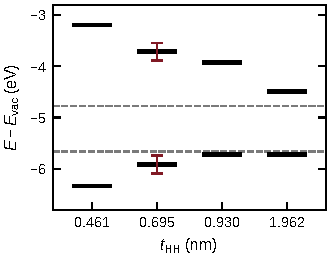
\includegraphics[width=\linewidth]{06_edges}
      \src{Upper bars $-$EA, lower bars $-$IP; dashed: bulk edges via the 2\,nm alignment. This work \sixlab{computed}.
        Maroon: $\pm0.17$\,eV vacuum-reference sensitivity of the polar film \sixlab{assumed}, not an error bound.}
    \end{column}
  \end{columns}
  \takeaway{Primary $\dEc$ law: 1 and 2\,nm films only; the polar film stays in the other laws.}
\end{frame}

% ---------------------------------------------------------------------------------------------------------------------
\begin{frame}{The gap opens by 0.34\,eV at 2\,nm and 0.90\,eV at 1\,nm}
  \sixdense
  \begin{columns}[T,onlytextwidth]
    \begin{column}{0.42\textwidth}
      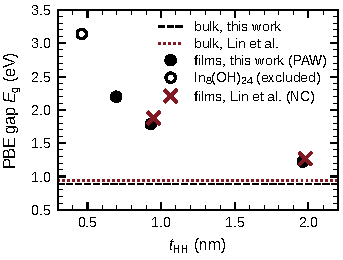
\includegraphics[width=\linewidth]{06_gaps}
      \src{PBE gaps. This work: PAW, 71\,Ry \sixlab{computed}. Crosses, dotted: Lin et al., norm-conserving, 140\,Ry,
        at their labels 0.95 and 1.98\,nm\sref[pp.~21540, 21542]{Lin2022}\xdef\sixlinfn{\the\value{footnote}}.}
    \end{column}
    \begin{column}{0.54\textwidth}
      \begin{itemize}
        \item Opening relative to the bulk PBE gap \lab{computed}:
          \begin{align*}
            \dEg(1.962\,\mathrm{nm}) &= 1.2239 - 0.8887 = 0.335\,\mathrm{eV}\\
            \dEg(0.930\,\mathrm{nm}) &= 1.7885 - 0.8887 = 0.900\,\mathrm{eV}
          \end{align*}
        \item Lin et al.\footnotemark[\sixlinfn], same recipe: $+0.33$\,eV at 1.98\,nm, $+0.94$\,eV at 0.95\,nm.
          Differences 0.005 and 0.04\,eV, inside the pre-registered 0.1\,eV \lab{derived}.
        \item Bulk and 1\,nm gaps and masses lie 4--7\,\% below theirs\footnotemark[\sixlinfn], all with one sign. This
          points to the numerical setup (PAW 71\,Ry against norm-conserving 140\,Ry) rather than to the films
          \lab{inferred}.
        \item Relaxation is essential: as built, the 1\,nm film opened the gap by only 0.07\,eV \lab{computed}.
      \end{itemize}
    \end{column}
  \end{columns}
  \takeaway{The 1 and 2\,nm openings reproduce an independent PBE study within 0.04\,eV.}
\end{frame}

% ---------------------------------------------------------------------------------------------------------------------
\begin{frame}{The gap law is well determined; the $\dEc$ law is not}
  \sixdense
  \begin{columns}[T,onlytextwidth]
    \begin{column}{0.38\textwidth}
      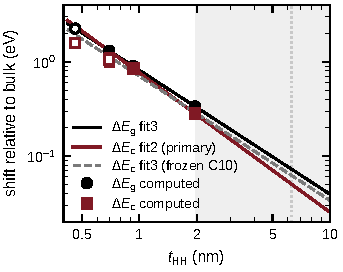
\includegraphics[width=\linewidth]{06_laws}
      \src{Open: 0.461\,nm (excluded); 0.695\,nm $\dEc$, bar: $\pm0.17$\,eV vacuum-reference sensitivity
        \sixlab{assumed}. Lines: $y = a\,t^{-p}$ \sixlab{fitted}; dotted: 6.3\,nm; grey: beyond the thickest film
        (extrapolation).}
    \end{column}
    \begin{column}{0.58\textwidth}
      \begingroup\scriptsize
      \renewcommand{\arraystretch}{1.05}
      \begin{tabular}{@{}l c c c@{}}
        \toprule
        law (points; $t = \tHH$ in nm) & $a$ (eV) & $p$ & 6.3\,nm (eV) \\
        \midrule
        $\dEg$ fit3 (0.695, 0.930, 1.962) & 0.815 & 1.316 & 0.072 \\
        $\dEc$ fit2, primary (0.930, 1.962) & 0.762 & 1.478 & 0.050 \\
        $\dEc$ fit3, frozen C10 (three points) & 0.702 & 1.318 & 0.062 \\
        \bottomrule
      \end{tabular}\par\endgroup
      \begin{itemize}
        \item $\dEg$: three points within 0.5\,\% of the law; leave-one-out $p = 1.29$--1.32 \lab{fitted};
          $\sigma_p = 0.007$ is scatter only (1 dof).
        \item $\dEc$: two clean points, no residual freedom. With the polar point $p = 1.32$ (leave-one-out
          0.76--1.48); moving it by $\mp0.17$\,eV gives 0.075 or 0.053\,eV at 6.3\,nm \lab{fitted}.
        \item A constant $\dEv \approx -0.053$\,eV lowers the $\dEg$ exponent (1.32 against 1.48): the laws are not
          interchangeable \lab{derived}.
        \item Every law is crystalline (001), PBE, one termination, used 3$\times$ beyond its data at 6.3\,nm; $\sigma$
          omits these errors and the untested field effect on the 0.695\,nm gap.
      \end{itemize}
    \end{column}
  \end{columns}
  \takeaway{$\dEc$ at 6.3\,nm is known only as a range, 0.050--0.075\,eV, set by the choice of fit.}
\end{frame}

% ---------------------------------------------------------------------------------------------------------------------
\begin{frame}{The conduction band takes 84 to 94\,\% of the gap opening}
  \sixdense
  \begin{columns}[T,onlytextwidth]
    \begin{column}{0.40\textwidth}
      {\centering
      \begin{tikzpicture}[x=1mm,y=1mm,font=\scriptsize]
        % energies relative to the bulk valence-band maximum, 15 mm per eV
        \draw[rulegrey,dashed,line width=0.5pt] (-1,0) -- (47,0);
        \draw[rulegrey,dashed,line width=0.5pt] (-1,13.33) -- (47,13.33);
        \node[anchor=east,inkgrey] at (-1,0) {$E_{\mathrm{v}}^{\mathrm{bulk}}$};
        \node[anchor=east,inkgrey] at (-1,13.33) {$E_{\mathrm{c}}^{\mathrm{bulk}}$};
        % bulk
        \draw[line width=1.3pt] (0,0) -- (12,0);
        \draw[line width=1.3pt] (0,13.33) -- (12,13.33);
        \draw[{Stealth[length=1.3mm]}-{Stealth[length=1.3mm]},line width=0.5pt] (4,0.4) -- (4,12.93);
        \node[anchor=west] at (4.5,6.7) {0.889};
        % 1.962 nm
        \draw[line width=1.3pt] (17,-0.81) -- (29,-0.81);
        \draw[line width=1.3pt] (17,17.55) -- (29,17.55);
        \draw[{Stealth[length=1.3mm]}-{Stealth[length=1.3mm]},line width=0.5pt] (20.5,-0.41) -- (20.5,17.15);
        \node[anchor=west] at (21.0,8.4) {1.224};
        \draw[-{Stealth[length=1.3mm]},ntumaroon,line width=0.8pt] (27.5,13.33) -- (27.5,17.35);
        \node[anchor=south] at (23,17.9) {$+0.281$};
        \node[anchor=north] at (23,-1.2) {$-0.054$};
        % 0.930 nm
        \draw[line width=1.3pt] (34,-0.78) -- (46,-0.78);
        \draw[line width=1.3pt] (34,26.05) -- (46,26.05);
        \draw[{Stealth[length=1.3mm]}-{Stealth[length=1.3mm]},line width=0.5pt] (37.5,-0.38) -- (37.5,25.65);
        \node[anchor=west] at (38.0,8.4) {1.789};
        \draw[-{Stealth[length=1.3mm]},ntumaroon,line width=0.8pt] (44.5,13.33) -- (44.5,25.85);
        \node[anchor=south] at (40,26.4) {$+0.848$};
        \node[anchor=north] at (40,-1.2) {$-0.052$};
        % column labels
        \node[anchor=north] at (6,-5.0) {bulk};
        \node[anchor=north] at (23,-5.0) {1.962\,nm};
        \node[anchor=north] at (40,-5.0) {0.930\,nm};
      \end{tikzpicture}\par}
      \src{To scale, eV. Black arrows: gaps; maroon: $\dEc$ (value above); $\dEv$ below each film. 2\,nm: two-step
        alignment; 1\,nm: 2\,nm value plus EA/IP differences. This work \sixlab{computed}.}
    \end{column}
    \begin{column}{0.56\textwidth}
      \begingroup\scriptsize
      \renewcommand{\arraystretch}{1.12}
      \setlength{\tabcolsep}{4.5pt}
      \begin{tabular}{@{}l c c c c@{}}
        \toprule
        film, alignment route & $\dEc$ & $\dEv$ & $\dEv$, EMA & CB share \\
        \midrule
        1.962\,nm, two-step & $+0.281$ & $-0.054$ & $-0.016$ & 0.84 / 0.95 \\
        \quad double average & $+0.287$ & $-0.049$ & & 0.86 \\
        0.930\,nm, 2\,nm + EA/IP & $+0.848$ & $-0.052$ & $-0.061$ & 0.94 / 0.93 \\
        \quad two-step$^{a}$ & $+0.819$ & $-0.081$ & & 0.91 \\
        \bottomrule
      \end{tabular}\par\endgroup
      \src{Energies in eV; CB share: DFT / EMA. $^{a}$No bulk-like interior; not used. EMA: Kane-consistent, hole
        energy $\varepsilon_1m_b/m_h$ with $\varepsilon_1 = \dEc(1+\alpha\dEc)$, $m_h = 3.2\,m_0$ (lightest)
        \sixlab{derived}.}
      \begin{itemize}
        \item Same termination: $\dEc(1) - \dEc(2) = \mathrm{EA}(2) - \mathrm{EA}(1) = +0.567$\,eV,
          $\dEv(1) - \dEv(2) = \mathrm{IP}(2) - \mathrm{IP}(1) = +0.002$\,eV \lab{computed}.
        \item EMA agrees at 1\,nm. At 2\,nm the computed $|\dEv|$ is about 38\,meV larger, beyond the route spread
          (5\,meV) and plateau flatness (8\,meV): unexplained \lab{unresolved}.
        \item The device model uses only $\dEc$ and the gap: $\dEv \approx -0.05$\,eV does not move the electron barrier.
      \end{itemize}
    \end{column}
  \end{columns}
  \takeaway{At 2\,nm the conduction band rises by 0.28\,eV; the V1 device model assumed 0.35\,eV.}
\end{frame}

% ---------------------------------------------------------------------------------------------------------------------
\begin{frame}{Envelope models bracket the shift but do not predict it}
  \sixdense
  \begin{columns}[T,onlytextwidth]
    \begin{column}{0.41\textwidth}
      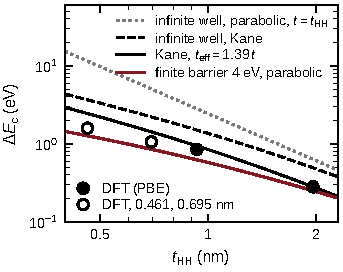
\includegraphics[width=0.96\linewidth]{06_models}
      \src{Bulk PBE $m_b = 0.1541\,m_0$, $\alpha = 0.58$\,eV$^{-1}$; dotted, dashed, maroon \sixlab{derived}. Solid:
        box $1.39\,\tHH$, fitted to the 1.962\,nm point \sixlab{fitted}.}
    \end{column}
    \begin{column}{0.55\textwidth}
      \begin{itemize}
        \item Infinite well, $t = \tHH$:
          $E_n - \Ec = \dfrac{\hbar^2\pi^2n^2}{2m_bt^2} = \dfrac{0.376\,\mathrm{eV\,nm^2}}{(m_b/m_0)\,t^2}\,n^2$\\
          0.634\,eV at 1.962\,nm, $2.3\times$ the computed value \lab{derived}.
        \item Kane band\sref{Kane1957}, $E(1+\alpha E) = \hbar^2k^2/2m_b$: the fitting box grows from $1.39\,\tHH$
          (1.962\,nm) to $1.49\,\tHH$ (0.930\,nm); fixed at 2\,nm it gives 0.94\,eV at 1\,nm, not 0.848
          \lab{derived}.
        \item 4\,eV barrier, $m_0$ outside, $F'/m$ continuous\sref{Bastard1981}: 0.25\,eV at 1.962\,nm, 0.63\,eV at
          0.930\,nm. The envelope leaks 0.6\,nm per side: the result rests on a boundary condition that is undetermined
          at an atomic surface \lab{derived}.
        \item The bixbyite cell is 1.03\,nm: the 1\,nm film is thinner than one cell, the 2\,nm film spans two. For
          every film here envelope theory is a parametrisation to be tested.
      \end{itemize}
    \end{column}
  \end{columns}
  \takeaway{Not refuted, but not predictive: the device model takes $\dEc$ from DFT, not from a box.}
\end{frame}

% ---------------------------------------------------------------------------------------------------------------------
\begin{frame}{HSE06 changes the 1\,nm gap opening by only 6 to 11\,\%}
  \sixdense
  \begin{columns}[T,onlytextwidth]
    \begin{column}{0.41\textwidth}
      \begingroup\scriptsize
      \renewcommand{\arraystretch}{1.12}
      \setlength{\tabcolsep}{3.5pt}
      \begin{tabular}{@{}l c c c@{}}
        \toprule
        Kohn--Sham gaps (eV) & bulk & 1\,nm film & $\dEg$ \\
        \midrule
        PBE & 0.9204 & 1.8068 & 0.8864 \\
        HSE06, $q = 1$ & 2.1080 & 3.0475 & 0.9395 \\
        \midrule
        ratio $r$ & & & 1.060 \\
        \bottomrule
      \end{tabular}\par\endgroup
      \src{SG15 norm-conserving\srefs{Hamann2013,Schlipf2015}, 80\,Ry, both functionals at the PBE geometries. Bulk PBE:
        VBM off $\Gamma$ (direct gap at $\Gamma$ 0.9216\,eV). This work \sixlab{computed}.}
      \vspace{2mm}
      \begingroup\scriptsize
      \renewcommand{\arraystretch}{1.12}
      \begin{tabular}{@{}c c@{}}
        \toprule
        HSE06 bulk mass $m_b$ ($m_0$) & Kane-model $r$ \\
        \midrule
        0.159 & 1.158 \\
        0.170 & 1.095 \\
        0.193 & 0.983 \\
        \bottomrule
      \end{tabular}\par\endgroup
      \src{Masses estimated from the HSE06 SCF grid; $r$ from a Kane band with $\alpha = 0.58\times0.920/2.108
        = 0.253$\,eV$^{-1}$ \sixlab{derived}.}
    \end{column}
    \begin{column}{0.56\textwidth}
      \begin{itemize}
        \item HSE06\srefs{Heyd2003,Heyd2006,Krukau2006} at fixed geometry, norm-conserving (PAW exact exchange had not
          finished its first step after 4.5\,h on an H100); only $r$ is transferred.
        \item $r = 1.060$ meets the pre-registered 10\,\% criterion; a $3\times3\times3$ exchange $q$ grid lowers the bulk
          HSE06 gap by 42\,meV, so $r = 1.06$--1.11 \lab{computed}.
        \item PAW and norm-conserving PBE openings agree within 1.6\,\% \lab{computed}: HSE-corrected 1\,nm opening
          0.95--1.00\,eV, gap 3.06\,eV \lab{derived}; 2\,nm gap 2.44--2.46\,eV if $r$ transfers (amendment A23)
          \lab{assumed}.
        \item Why $r\approx1$: HSE06 makes the band heavier but less non-parabolic; a Kane band with
          $\alpha\propto1/\Eg$ (assumed) gives 0.98--1.16, bracketing $r$ without deriving it \lab{derived}.
      \end{itemize}
    \end{column}
  \end{columns}
  \takeaway{PBE misses the gap but not the 1\,nm shift; other thicknesses assume the same $r$.}
\end{frame}

% ---------------------------------------------------------------------------------------------------------------------
\begin{frame}{One subband at 2\,nm, but not reliably at 6.3\,nm}
  \sixdense
  \begin{columns}[T,onlytextwidth]
    \begin{column}{0.42\textwidth}
      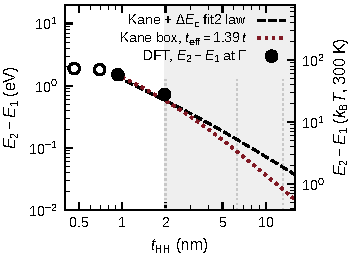
\includegraphics[width=\linewidth]{06_subbands}
      \src{Spacing $E_2-E_1$ of the lowest two conduction levels at $\Gamma$: DFT (open: 0.461, 0.695\,nm)
        \sixlab{computed}; Kane estimates \sixlab{derived}. Dotted: device thicknesses 2.0, 6.3 and 13.2\,nm; grey:
        beyond the thickest film (extrapolation).}
    \end{column}
    \begin{column}{0.54\textwidth}
      \begin{itemize}
        \item Crystalline films, PBE: $E_2 - E_1 = 0.72$\,eV at 1.962\,nm and 1.50\,eV at 0.930\,nm;
          $(E_2-E_1)/E_1 = 2.56$ and 1.77, below the parabolic 3 \lab{computed}.
        \item One occupied subband needs $E_2 - E_1 \gg \kT$. Kane band with the $\dEc$ law: 0.59\,eV ($23\,\kT$) at
          1.962\,nm, 0.14\,eV ($5\,\kT$) at 6.3\,nm, 0.05\,eV ($2\,\kT$) at 13.2\,nm \lab{derived}.
        \item The 6.3 and 13.2\,nm values extrapolate the law 3 to 7 times; a box of width $1.39\,t$ gives
          0.088\,eV ($3.4\,\kT$) at 6.3\,nm \lab{derived}. Degenerate filling is ignored.
        \item The device films are amorphous or nanocrystalline: whether this transfers is registered test H-K
          (Part 11).
      \end{itemize}
    \end{column}
  \end{columns}
  \takeaway{Estimate for a crystalline PBE film: one subband at 2\,nm, one or two at 6.3\,nm, several at 13\,nm
    \lab{derived}.}
\end{frame}
